\documentclass[tikz,border=2pt]{standalone}
\usepackage{amsmath}
\usepackage{pgfplots}
\pgfplotsset{compat=1.18}

\begin{document}
% An increasing sequence that is bounded above converges, to the supremum of its terms:
% a_n = 2 - 3/(n+1) climbs towards sup{a_n} = 2 and never crosses the bound M = 2.3.
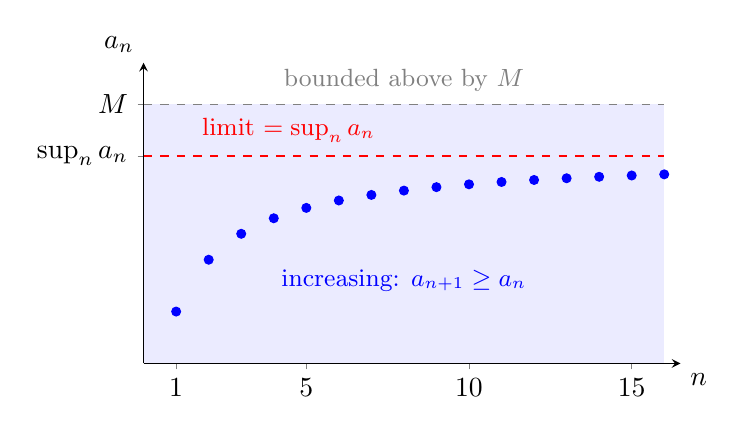
\begin{tikzpicture}
	\begin{axis}[
		axis lines=middle,
		xmin=0, xmax=16.5,
		ymin=0, ymax=2.9,
		xtick={1,5,10,15}, ytick={2,2.5}, yticklabels={$\sup_n a_n$,$M$},
		xlabel={$n$}, ylabel={$a_n$},
		xlabel style={below right}, ylabel style={above left},
		clip=false,
		width=8.4cm, height=5.4cm
		]
		\fill[blue!8] (axis cs:0,0) rectangle (axis cs:16,2.5);
		\addplot[gray, dashed, domain=0:16] {2.5};
		\addplot[red, dashed, domain=0:16] {2};
		\addplot[only marks, mark=*, mark size=1.6pt, blue, samples at={1,...,16}] {2-3/(x+1)};
		\node[blue, anchor=north, font=\small] at (axis cs:8,1.0) {increasing: $a_{n+1}\ge a_n$};
		\node[gray, anchor=south, font=\small] at (axis cs:8,2.53) {bounded above by $M$};
		\node[red, anchor=south west, font=\small] at (axis cs:1.5,2.04) {limit $=\sup_n a_n$};
	\end{axis}
\end{tikzpicture}
\end{document}
